\section{Attacking the result: nine objections and what the data say}\label{sec:objections}

Throughout the research we raised nine objections to this ten-stock backtest that are tested here (Table~\ref{tab:objections}). Tests on the strategy use the frozen specification. Tests on the research process use the full family of reasonable specifications. The code is \texttt{scripts/reproduce\_audit.py} in the repository and Block 17 of the notebook.

\begin{table}[t]
\centering\scriptsize
\caption{Anticipated objections, the test applied and the verdict}\label{tab:objections}
\begin{adjustbox}{max width=\textwidth}\begin{tabular}{p{0.24\textwidth}p{0.29\textwidth}p{0.39\textwidth}}
\toprule
Objection & Test & Result\\
\midrule
1. The universe was chosen with hindsight, the book is long the later winners. & Lo (2008) decomposition, causal static and timing books, partial pooling of per-stock P\&L & The timing book carries the edge (Sharpe 1.04, $t = 2.41$, never-seen 1.33, $t = 2.21$). The static tilt is insignificant and negative out of sample.\\
2. Execution at the signal close and free shorting are unrealistic. & 0-2 session delay $\times$ 0-200\,bp borrow $\times$ 0-30\,bp costs, breakeven cost & Sharpe 0.96 (0.89 never-seen) in the harshest cell, breakeven cost 234\,bp per unit traded.\\
3. Overlapping tranches smooth P\&L and inflate the Sharpe ratio. & Lo (2002) autocorrelation-adjusted Sharpe & 1.06 and 1.06, first-order autocorrelation 0.04.\\
4. Zero average beta hides crash beta. & Up- and down-market betas, worst market weeks & Down-market beta $-0.07$ ($t = -1.24$), positive mean return in the worst market decile.\\
5. The parameters were chosen to make it work. & Multiverse of $\approx$300 specifications, SPA, PBO, selection-free ensemble & 99\% (97\%) of specifications earn a positive Sharpe, the ensemble earns 0.92 ($t = 1.97$) and 0.86.\\
6. Beating the toolkit is cherry-picking. & Romano-Wolf step-down against 16 books, reverse SPA & No comparable beats FMF-N (SPA $p = 0.86$, 0.86), FMF-N significantly beats 2 books after FWER control in sample.\\
7. The new signal adds nothing to classic breadth. & FMF-N vs the same book without LMH, pooled across samples & $+0.28$ Sharpe ($p = 0.028$) in sample, $+0.30$ out of sample, $P(\text{gain}>0) = 0.94$ pooled.\\
8. Ten stocks and a few years prove nothing. & Bayesian Sharpe under sceptical priors, random-effects meta-analysis, empirical-Bayes shrinkage, Bayes factors, power & $P(IC>0$ in the next universe$) = 0.96$, pooled IC 0.105, Stouffer $p = 0.0022$, the 18-signal search shrinks LMH's $t$ to 1.06.\\
9. One history has one drawdown. & Generative stress tests (bootstrap, FHS, Diffusion-FHS, TimeGAN) with posterior-predictive drift & Five-year median Calmar 0.70, 5\% max drawdown $-34\%$, the binding stress is a momentum crash (5\% three-month quantile about $-15\%$), not a market crash.\\
\bottomrule
\end{tabular}\end{adjustbox}
\par\smallskip\begin{minipage}{0.95\textwidth}\scriptsize Development: 2017-2021, 10 US large caps. Never-seen period: 2024-01-05 to 2026-08-05, 30 stocks (20 never used in development). Details in Sections~\ref{sec:identity}-\ref{sec:generative}.\end{minipage}
\end{table}

\subsection{Identity or timing?}\label{sec:identity}

Hindsight is the most serious objection to a backtest on a named universe. The ten development stocks are well-known large caps whose 2016-2021 paths were known when the universe was put together. A book that is on average long the names that later did well makes money with no timing skill at all, and the circular time-shift placebo of Section~\ref{sec:results}, which keeps each stock's habitual rank, cannot exclude this. \citet{lo2008} gives the decomposition. For a book with weights $w_{i,t}$ the mean return is
\begin{equation}
E\Big[\sum_i w_{i,t-1}r_{i,t}\Big]=\underbrace{\sum_i \operatorname{Cov}(w_{i,t-1},r_{i,t})}_{\text{active: timing}}+\underbrace{\sum_i E[w_{i,t-1}]\,E[r_{i,t}]}_{\text{passive: identity}}.\label{eq:lo}
\end{equation}
Because the passive term is computed with averages over the whole window, I use it only as a diagnostic. For the test itself I split the book in two tradable parts. The static book holds $\bar w_{i,t}=\tfrac1t\sum_{s\le t}w_{i,s}$, the running mean of each stock's past weights. The timing book holds the rest, $w_{i,t}-\bar w_{i,t}$. Their sum is the strategy, and neither uses future data.

The result is clear (Figure~\ref{fig:identity}). In the development universe the timing book earns 8.9\% a year with a Sharpe ratio of 1.04 ($t_{\text{HAC}} = 2.41$), the static book earns 2.2\% ($t = 1.08$). Over the never-seen period the gap widens: timing has a Sharpe ratio of 1.33 ($t = 2.21$) and the static tilt loses money (Sharpe $-0.49$). The edge is in when the revision flow turns, not in which stocks it usually favours. The time-shift placebo is best read as a test with low power. Its null distribution is wide because shifted signals keep their slow structure, not because identity explains the returns.

A Bayesian partial-pooling model of per-stock P\&L contributions (normal-normal, cross-stock heterogeneity estimated) confirms that the development result is not one name. The largest contributor (stock\_6, 5.7\% a year) shrinks to 4.5\%, and the posterior probability that the typical stock contributes positively is 0.87. Out of sample the contributions are small and spread over the 30 names. Ten of these names are development stocks, on the other twenty alone the frozen book has a Sharpe ratio of 0.80 and LMH an IC of 0.105 (Section~\ref{sec:oos}), so the out-of-sample timing edge does not come from names already studied.

\begin{figure}[t]
\centering
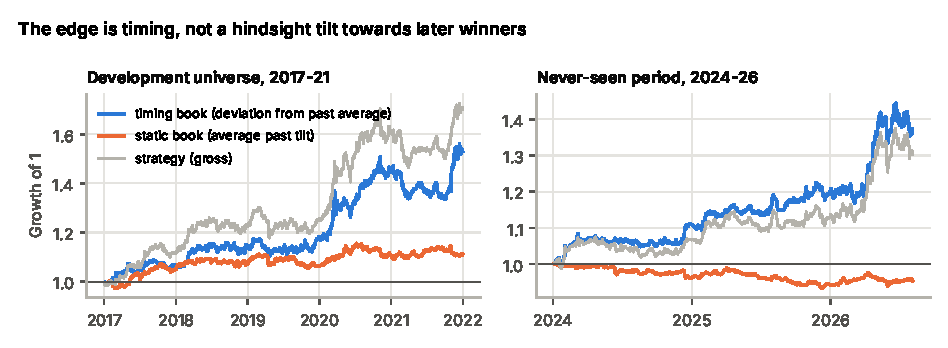
\includegraphics[width=\figw]{fig/fig13.pdf}
\caption{Causal decomposition of the gross book into a static book (each stock's expanding average of past weights) and a timing book (today's deviation from it). Both are tradable and add up to the strategy.}\label{fig:identity}
\end{figure}

\subsection{Implementation: delay, borrow, costs, smoothing and crash beta}

Four practical objections decide whether a paper alpha becomes a live loss. Table~\ref{tab:objections} and Figure~\ref{fig:implementation} report the full grid.
\begin{itemize}
  \item \emph{Execution delay:} Trading one session after the signal close leaves the development Sharpe ratio at 1.13, because each day only one forty-second of the book is re-targeted, a day's delay does not front-run information that builds over weeks
  \item \emph{Borrow and costs:} With a one-session delay, 10\,bp per unit traded and a 100\,bp annual borrow fee on all short notional, the Sharpe ratio is 1.06 (0.99 over the never-seen period). In the harshest cell of the grid (two sessions, 200\,bp borrow, 20\,bp costs) it is 0.96 and 0.89. The breakeven cost per unit traded is 234\,bp (197\,bp), the cleanest capacity diagnostic available without volume data and an order of magnitude above the cost of trading liquid large caps
  \item \emph{Smoothing:} Overlapping tranches smooth positions and not returns. The first-order autocorrelation of daily P\&L is 0.04 and the \citet{lo2002} autocorrelation-adjusted Sharpe ratio is 1.06 (1.06)
  \item \emph{Crash beta:} Weekly regressions with separate up- and down-market slopes give a down-market beta of $-0.07$ ($t = -1.24$) and an up-market beta of 0.03. In the worst decile of market weeks the book's average return is positive
\end{itemize}

\begin{figure}[t]
\centering
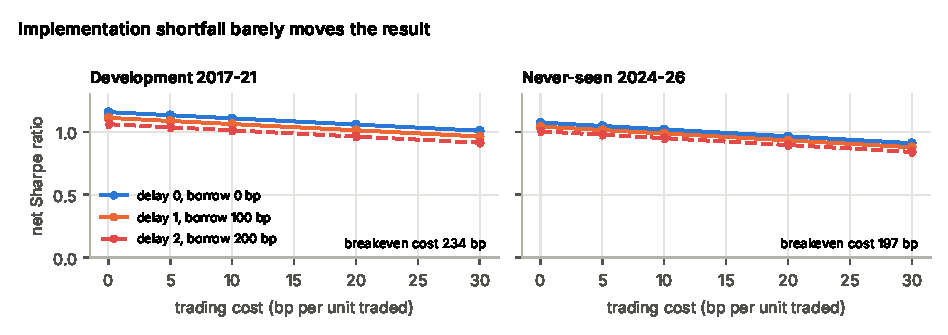
\includegraphics[width=\figw]{fig/fig14.pdf}
\caption{Net Sharpe ratio against trading cost in three implementation regimes: at the signal close without borrow fees, one session late with a 100\,bp borrow fee, two sessions late with a 200\,bp borrow fee.}\label{fig:implementation}
\end{figure}

\subsection{Research degrees of freedom}

A backtest has many choices (windows, thresholds, legs, tranches, allocators, signal sets, data rules), a result valid for one combination only is a search artefact. In the spirit of the multiverse analysis of \citet{steegen2016} and the specification curve of \citet{simonsohn2020}, I run the whole pipeline again over every choice in this research space. The grid covers the leader gap (5-20), the herd window (2-10 to 5-20), the LMH window (63-252), the breadth window, tranche length, legs, allocator, four signal sets, the information-event threshold (4-6), a two-session knowledge lag and the target expiry. The expiry choices include the quarterly 63-session horizon of the earnings cycle, as well as 126 and 252 sessions. Each parameter is moved one at a time, and 300 joint specifications are drawn at random.

Figure~\ref{fig:multiverse} shows three results.
\begin{itemize}
  \item \emph{The sign is not a choice:} 99\% of the development specifications and 97\% of the never-seen ones have a positive net Sharpe ratio (medians 0.80 and 0.72). The frozen specification is at the 98th percentile in development, as selection would imply, and at the 83rd out of sample, which selection would not
  \item \emph{The level depends on the choice:} Rankings inside the family do not persist (PBO 0.76). The ensemble of all specifications (no selection) has a Sharpe ratio of 0.92 over 2017-2021 ($t = 1.97$) and 0.86 out of sample, about 0.8 times the frozen specification
  \item \emph{Quarterly calibration and knowledge lag:} A hard 63-session expiry lowers the development Sharpe ratio to 0.94 (0.88 out of sample): dropping a target after one quarter throws away the information from analysts who update twice a year. Expiry at 126 sessions is equivalent to the 252-session default (1.12, 1.15). A two-session knowledge lag changes nothing (1.13, 1.06). Staleness is better handled inside the signal, by the event and silence clocks of LMH, than by cutting the snapshot short
\end{itemize}
Hansen's \citeyearpar{hansen2005} SPA test on a single window does not reject the null that no specification beats zero (development $p = 0.34$, never-seen $p = 0.14$, 2017-2021 ensemble $p = 0.095$). Section~\ref{sec:bayes} therefore combines the independent samples.

\begin{figure}[t]
\centering
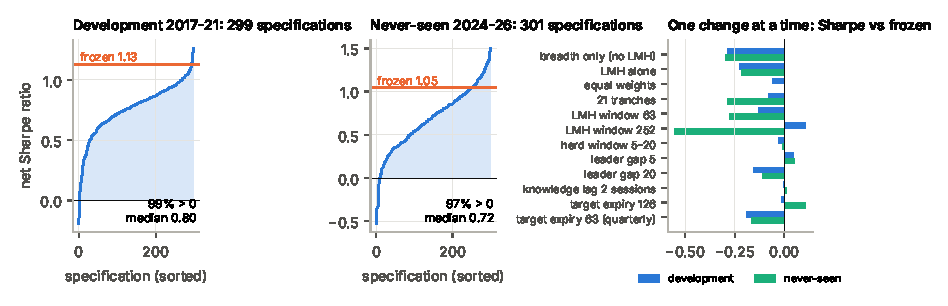
\includegraphics[width=\figw]{fig/fig15.pdf}
\caption{Left and centre: specification curves, i.e.\ the net Sharpe ratio of every randomly drawn specification sorted from worst to best, with the frozen specification marked. Right: change in Sharpe ratio when one choice at a time moves away from the frozen specification.}\label{fig:multiverse}
\end{figure}

\subsection{Multiple testing against the toolkit, and the marginal value of LMH}

Ranking first of 14 cross-sectional books (Section~\ref{sec:toolkit}) invites a charge of cherry-picking the comparison set. Two family-wise tests deal with it. The reverse SPA test asks whether any of the 16 institutional books significantly beats FMF-N once all are scaled to the same volatility, none does ($p = 0.86$ in sample, 0.86 out of sample). The \citet{romano2005} step-down procedure asks which books FMF-N beats under family-wise error control. In sample it beats 2 of 16, among them target-price momentum and 6-1 momentum. Out of sample no difference survives the correction, though 2 are individually significant. The defensible claim is ``never beaten, and better than most'', not ``significantly better than everything''.

The harder question is whether the new signal earns its place. Classic revision breadth is FMF's closest relative (correlation of the books 0.95). I compare FMF-N with the identical book built from the three breadth signals only, using a circular block bootstrap of paired returns \citep{ledoit2008}, the high correlation of the two books is what gives the test power. LMH adds 0.28 to the Sharpe ratio in development (95\% interval 0.03 to 0.54, $p = 0.028$) and 0.30 over the never-seen period ($-0.21$ to 0.80). Pooled, the gain is 0.29, with a posterior probability of 0.94 that it is positive.

\subsection{Small samples, done properly}\label{sec:bayes}

A $p$-value measures how surprising the data are under an effect of exactly zero. It ignores two facts an allocator would use. Most strategies fail, and here the same mechanism shows up in three independent samples, each with its own analysts and its own market path. Four Bayesian and small-sample tools are used (Figure~\ref{fig:bayes}).

\para{Posterior Sharpe ratios under sceptical priors:} The Bayesian bootstrap \citep{rubin1981} of weekly returns is a nonparametric posterior in which skewness and fat tails enter through the data, it is re-weighted by a prior on the annual Sharpe ratio. Under a sceptical $N(0,1)$ prior (most strategies have $|SR|<2$) the 2017-2021 posterior mean is 1.00 with $P(SR>0)=0.99$. Over the never-seen period it is 0.76 with $P(SR>0)=0.93$. Under a very sceptical $N(0,0.5)$ prior, which encodes the post-publication decay of anomalies documented by \citet{mclean2016}, the probabilities are 0.97 and 0.86.

\para{Random-effects meta-analysis across independent samples:} Development, holdout and the never-seen period are three non-overlapping samples of the same mechanism (the third adds twenty new names to the ten development names). A normal-normal random-effects model with a half-Cauchy prior on the between-sample heterogeneity $\tau$ \citep{gelman2006} pools them without assuming one common true effect. The LMH information coefficients are 0.095, 0.129 and 0.096. The pooled mean is 0.105 (90\% HDI 0.033 to 0.179), and the posterior-predictive probability of a positive IC in the next universe is 0.96. Stouffer's combination of the three one-sided $p$-values gives $p = 0.0022$, and the product of the three Bayes factors (prior sd 0.1) is 22. For the strategy's Sharpe ratio the pooled mean is 1.10 (90\% HDI 0.36 to 1.84), with $P(SR>0$ in the next universe$)=0.96$ and $P(SR>0.5)=0.86$.

\para{Shrinking the search:} In development LMH was the best of 18 candidate signals (Fama-MacBeth $t = 2.46$). Empirical-Bayes (James-Stein) shrinkage of the 18 $t$-statistics towards their family \citep{efron2010} brings this down to 1.06, with a posterior probability of 0.95 of a positive effect. This is what the development search is worth on its own: suggestive, not conclusive. It becomes evidence because the holdout and the never-seen period, which had no role in the search, gave the same information coefficient.

\para{Power:} With $N$ stocks and $M$ independent monthly cross-sections, the smallest mean IC detectable at 80\% power is $(z_{0.95}+z_{0.80})/\sqrt{(N-1)M}$ (Figure~\ref{fig:power}): 0.138 for ten stocks over three years, 0.077 for thirty, and 0.032 for a hundred stocks over five years. One ten-stock sample has a coin-flip chance (0.56) of detecting an IC of 0.10, so a null result in such a sample would tell us little. The never-seen period raises power to 0.91 and the three pooled samples go above 0.99. Monte Carlo on the calibrated generator agrees: with a true effect of the size in the data, the full pipeline finds it in 0.45 of ten-stock five-year worlds and 0.70 of thirty-stock worlds.

\begin{figure}[t]
\centering
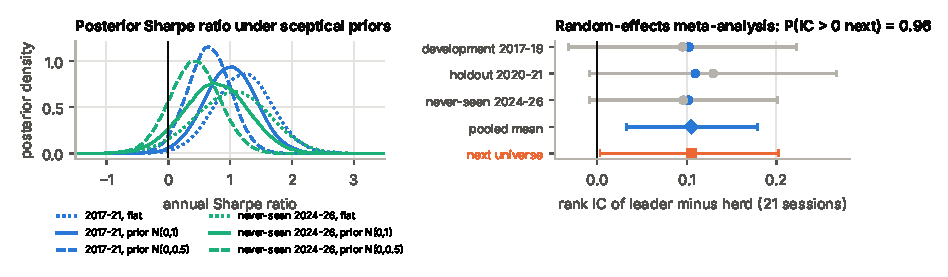
\includegraphics[width=\figw]{fig/fig16.pdf}
\caption{Left: posterior distributions of the annual Sharpe ratio (Bayesian bootstrap of weekly returns) under a flat prior and two sceptical priors. Right: random-effects meta-analysis of the leader-minus-herd IC. Grey: sample estimates with 95\% intervals, blue dots: partially pooled estimates, diamond: pooled mean (90\% HDI), square: predictive IC in a new universe.}\label{fig:bayes}
\end{figure}

\begin{figure}[t]
\centering
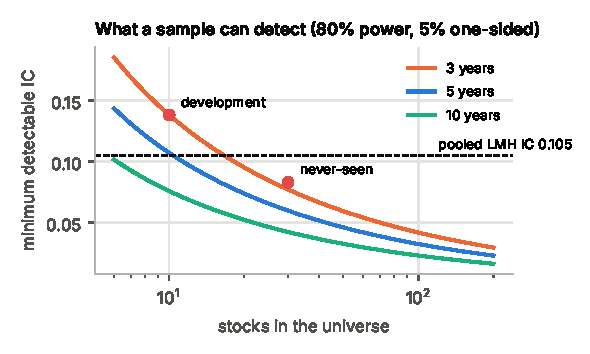
\includegraphics[width=0.62\textwidth]{fig/fig17.pdf}
\caption{Minimum detectable mean IC (80\% power, one-sided 5\%) by universe size and sample length. Red dots: the two universes of this paper. Dashed: the pooled LMH IC.}\label{fig:power}
\end{figure}
